% ZK-Duel paper. Build: paper\build.cmd. Checks: python paper/check.py
% Every line with a number carries "% src: <file>"; check.py confirms each number occurs in that file.
\documentclass[conference]{IEEEtran}
\IEEEoverridecommandlockouts
\usepackage[T1]{fontenc}
\usepackage{cite}
\usepackage{amsmath}
\usepackage{graphicx}
\usepackage{booktabs}
\usepackage{url}
\usepackage{balance}
\newcommand{\status}[1]{\texttt{#1}}
\newcommand{\rmax}{r_{\max}}
\emergencystretch=1.5em

\begin{document}

\title{Commit, Challenge, Audit: Zero-Knowledge Proofs for Verifiable Fair Play in Real-Time Games}

\author{\IEEEauthorblockN{Shivansh Saroha}
\IEEEauthorblockA{\textit{Dept. of CSE}\\
\textit{The NorthCap University}\\
Gurugram, India\\
\textless email\textgreater}
\and
\IEEEauthorblockN{Vandana}
\IEEEauthorblockA{\textless designation\textgreater\\
\textit{Dept. of CSE}\\
\textit{The NorthCap University}\\
Gurugram, India}
}

\maketitle

\begin{abstract}
Anti-cheat systems for online games rely on privileged client software or on statistical detection, and neither produces evidence that a third party can check.
We investigate whether zero-knowledge proofs can supply such evidence for per-tick game rules in a real-time game.
We present a commit--challenge--audit protocol: a client commits to its hidden weapon state at the end of every window of ticks, the server spot-checks random windows during play, and all remaining windows are proven after the match.
We implement it in ZK-Duel, a browser-based 1v1 shooter, using Circom and snarkjs.
On one mid-range laptop, Groth16 takes 1.25~s in Chrome to prove a 1~s window, so sampling is necessary; % src: docs/REPORT.md
PLONK is 170--320 times slower and impractical. % src: docs/REPORT.md
In 135 scripted matches, all 124 with a rule-breaking cheat ended \status{audited\_failed}, % src: docs/REPORT.md
and 34 of 40 single-window cheats were caught live, against a naive estimate of 55\%; % src: docs/REPORT.md
median live detection latency was 4.5~s. % src: docs/REPORT.md
A smooth aimbot that stays within the rules ended \status{audited\_clean} in 11 of 11 matches. % src: docs/REPORT.md
Proofs establish rule compliance, not input provenance.
All results are from scripted bots on one machine.
\end{abstract}

\begin{IEEEkeywords}
zero-knowledge proofs, zk-SNARK, Groth16, PLONK, online games, anti-cheat, commitments, spot-checking, verifiable computation
\end{IEEEkeywords}

% ======================================================================
\section{Introduction}

Competitive online games depend on every player following the same rules.
Current defences give weak evidence of that.
Kernel-level drivers run with full system privileges, and some of them exhibit rootkit-like behaviour~\cite{dorner2024}.
Cheats nevertheless exist for every game in one recent study of competitive shooters~\cite{collins2024}.
Behavioural classifiers need access to gameplay data and produce a statistical judgement, and generated aimbots can be built to evade them~\cite{kanervisto2023}.
In both cases a player who is accused, or an opponent who has lost, must trust the vendor.
Neither approach yields evidence that a third party can re-check.

Zero-knowledge proofs (ZKPs)~\cite{gmr1989} offer a different kind of evidence: a client can show that it followed a rule without revealing the private state it used.
A recent review names this as a direction for future work and identifies proof generation time as the obstacle in fast-paced real-time settings~\cite{kapur2026}.
To the best of our knowledge, the cost of proving per-tick game rules against the time budget of a real-time game has not been measured, and no protocol for doing so has been evaluated against scripted cheats.

This paper makes the following contributions:
\begin{itemize}
\item A \emph{commit--challenge--audit} protocol that fixes a client's hidden state in every window, spot-checks random windows live and proves all remaining windows after the match, with explicit verdict rules for the recorded result.
\item ZK-Duel, a working browser-based 1v1 shooter that runs the protocol with a client-side prover in a Web Worker and a server-side verifier pool.
\item A measured comparison of Groth16 and PLONK on the same circuits and inputs, against the play time of each window, in Node and in Chrome.
\item A detection experiment over 135 matches, including a rule-abiding control, showing that the usual independent-sampling estimate is a lower bound on live detection and that spot-checks alone do not give a guarantee. % src: docs/REPORT.md
\end{itemize}

% ======================================================================
\section{Background and Related Work}

\subsection{Anti-Cheat Approaches}
A recent systematic review divides defences into server-side detection, client-side anti-tamper, kernel-level drivers and hardware-assisted trusted execution environments (TEEs), and weighs their effectiveness against overhead, privacy and scalability~\cite{alangari2025}.
Comparative and critical studies examine these methods, their intrusiveness and the effectiveness of client-side defences~\cite{lehtonen2020,gjonbalaj2023,dorner2024,collins2024}.
Capability-based client architectures aim to reduce the exploitable surface of the client itself~\cite{oster2025}.

\emph{Behavioural detection} classifies player traces with statistical or learned models~\cite{laurens2007,pao2010,alayed2013,pinto2021,loo2025,dhinge2026}.
BotScreen runs its detection in a distributed fashion on clients~\cite{choi2023}, and vision-based detectors look for illicit overlays in the frame buffer~\cite{jonnalagadda2021}.
Public datasets and cheat-injection frameworks support this line of work~\cite{bertin2026,shaikh2025}.
These methods address what proofs cannot, namely input automation, but their output is a judgement and not a checkable statement.

\emph{Hardware isolation} confines sensitive game logic in a TEE, for example to block wallhacks~\cite{park2020}, to harden a detection engine~\cite{brandao2020} or to protect mobile games~\cite{jeon2021}.
It requires trust in the hardware vendor.

\emph{Execution checking} is closest to our work.
Bethea et~al.\ check whether a client's message sequence can be explained by valid execution of the sanctioned client, using symbolic execution and constraint solving~\cite{bethea2011}.
Accountable virtual machines let users audit a logged execution, with online games as a motivating case~\cite{haeberlen2010}.
Joens et~al.\ supply game state to behaviour-based sensors through a trusted referee in low-trust settings~\cite{joens2024}.
None of these yields a succinct proof: the first has the operator solve constraints over the client's message history, the second has the auditor check a log of the execution, and the third relies on the referee.
Our verifier checks a short proof per window and does not learn the committed hidden state.

\subsection{Zero-Knowledge Proofs}
Goldwasser, Micali and Rackoff introduced the notion of knowledge complexity~\cite{gmr1989}.
Groth16 is a pairing-based succinct non-interactive argument whose proofs are small and fast to verify, at the price of a circuit-specific trusted setup~\cite{groth2016}.
PLONK uses a universal, updatable setup instead~\cite{plonk2019}.
Poseidon is a hash function designed to be cheap inside such circuits~\cite{poseidon2021}.
We write circuits in Circom~\cite{circom2023} and prove them with snarkjs~\cite{snarkjs}.
A recent empirical comparison of Groth16 and zk-STARKs targets a consumer-grade ARM platform and does not consider game time budgets~\cite{nainwal2025}.

\subsection{Zero-Knowledge Proofs in Games}
Baughman et~al.\ gave an early ZK protocol for games, which lets players confirm that they are within a given range of each other without learning their distance~\cite{baughman2007}.
On-chain hidden-information games such as Dark Forest\footnote{\url{https://blog.zkga.me/announcing-darkforest}} use zk-SNARKs for a cryptographic fog of war, with proofs checked on a blockchain and not against a per-tick time budget.
To the best of our knowledge, no prior work proves per-tick movement, aim and weapon rules for a real-time shooter or reports its detection performance.

% ======================================================================
\section{Threat Model and Fairness Claims}

\subsection{Attacker}
The attacker is a player with full control of their own machine.
They may modify the client, its memory and every message it sends, and they may withhold messages.
The server is trusted to run the protocol, draw challenges honestly and compute hits, and a dishonest server is outside the threat model.
We assume that the party who ran the circuit setup does not forge proofs (Section~\ref{sec:discussion}).

\subsection{Public and Hidden State}
Each tick, a client sends a public snapshot $(x, y, \mathit{angle}, \mathit{fired})$, which the server broadcasts.
The hidden state is the ammunition count, the cooldown, the reload timer, the reload input and the salts, and it never leaves the client in plaintext.
Hiding is partial: because \emph{fired} is public, an observer can estimate ammunition and cooldown, and only reload timing and salts stay truly hidden.

\subsection{What Is Proven}
For one window of $N$ ticks, a valid proof shows that the prover knew private values such that:
\begin{enumerate}
\item the public snapshots hash to the window's \emph{digest};
\item movement stayed within the per-axis speed limit and the arena bounds on every tick;
\item the shortest-arc turn stayed within the turn-rate limit on every tick;
\item the weapon followed its state machine: a 10-round magazine, a 12-tick cooldown and a 90-tick reload; % src: bench/out/screenshots/cheat-test-both-2026-10-23/README.md
\item the hidden state chains from commitment \emph{commitIn} to commitment \emph{commitOut}; and
\item the proof belongs to this match, player, round and window (\emph{bind}).
\end{enumerate}

\subsection{Out of Scope}
\emph{Hits are server-authoritative.} Hits, damage and round outcomes are computed by the server and are not proven.
\emph{Input provenance is not proven.} A proof shows that inputs obeyed the rules, not that a human produced them, so an aimbot that respects the turn limit is legal under every proven rule.
Information leaks are also out of scope: opponent positions are public by design, and the arena has no interior walls.

% ======================================================================
\section{Protocol Design}

Fig.~\ref{fig:arch} shows the components and messages.

\begin{figure}[t]
\centering
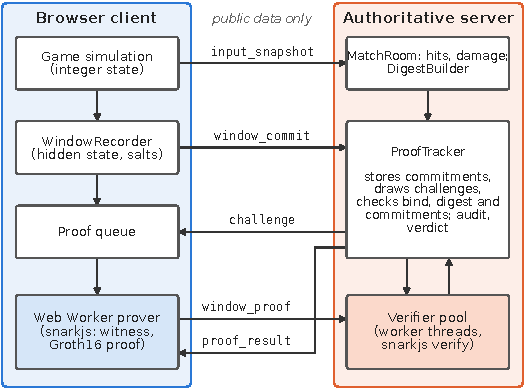
\includegraphics[width=\columnwidth]{figures/architecture.pdf}
\caption{ZK-Duel architecture. Only public snapshots, commitments and proofs cross the network. The server recomputes the digest from the snapshots it received.}
\label{fig:arch}
\end{figure}

\paragraph*{Windows}
Play is divided into rounds, and a round into windows of $N$ ticks at 60 ticks per second. % src: bench/RESULTS.md
A window covers $N/60$~s of play. % src: bench/RESULTS.md
The live default is $N=60$. % src: docs/REPORT.md

\paragraph*{Commitments}
When window $k$ ends, the client draws a fresh random salt and sends $\mathit{commitOut}_k = \mathrm{Poseidon}(\mathit{ammo}, \mathit{cooldown}, \mathit{reload}, \mathit{salt})$ over its last hidden state.
The server stores this claimed value and never accepts a replacement.
The chain starts each round from a public \emph{initialCommit} over the known starting state.

\paragraph*{Bind and digest}
Each proof has the public signals \emph{bind}, \emph{digest}, \emph{commitIn} and \emph{commitOut}.
$\mathit{bind} = \mathrm{Poseidon}(\mathit{matchField}, \mathit{player}, \mathit{round}, k)$ prevents replay across matches, players, rounds and windows.
The digest is a Poseidon chain over the window's snapshots.
The server computes it independently from the snapshots it actually received, so a client cannot prove one trajectory and send another.

\paragraph*{Random challenges}
Each player has at most one outstanding challenge.
The server draws it with a cryptographic random generator, uniformly among that player's windows in the current round that have ended, have a final digest and are still \status{committed}.
Because each candidate's commitment is fixed before the draw, a client cannot choose what to prove after learning which window was chosen.
A proof is accepted only if bind, digest, \emph{commitIn} (the claim for $k-1$) and \emph{commitOut} (the claim for $k$) all match, and the proof then verifies. % src: formula

A rewritten state, such as a refilled magazine, must occur inside some committed window, and that window then has no valid proof.
This is an informal argument, and we rely on the experiments and circuit tests to support it, not on a formal proof.
A window whose rules were broken is \status{unprovable}: witness generation aborts, so the client cannot produce a proof.
Our clients report this immediately.
A modified client could stay silent instead, which gives \status{timeout} when challenged and \status{unaudited} in the audit, and neither can end clean.

\paragraph*{Post-match audit}
After the match, the client proves every window that is still \status{committed}, one at a time, and the server verifies each proof in the same way.
A player or match is \status{audited\_clean} only if every window verified, \status{audited\_failed} if any window failed, and \status{audit\_incomplete} if any is missing.
The audit is what makes the guarantee complete, because spot-checks are only probabilistic.

\paragraph*{Enforcement and verdict rules}
In \emph{strict} mode, the first live failure ends the match with \status{forfeit\_proof}.
In \emph{observe} mode, failures are only recorded.
Audit results never rewrite the recorded winner, score or end reason.
The verdict depends only on the recorded winner's audit: \status{verified} if it is clean, \status{overturned} if it failed, and \status{unverified} if it is incomplete.

% ======================================================================
\section{Implementation}

ZK-Duel is a TypeScript monorepo with a browser client, a Node server and a shared rule module.
The same integer-only simulation code drives the client, the server's sanity checks and the generation of test vectors, so that the simulation and the circuit agree.
The circuit only checks and never clamps.
The server keeps match and proof records in SQLite.

\paragraph*{Circuit}
One Circom template, compiled with \texttt{--O2}, checks one window. % src: docs/REPORT.md
Range checks bound every comparator input to avoid field wrap-around.
Table~\ref{tab:circuit} gives the sizes, which grow linearly with $N$.
PLONK needs about 16--17 times as many constraints as R1CS, because every gate, including additions, becomes a row. % src: docs/REPORT.md
Groth16 uses the public Hermez Powers-of-Tau ceremony for phase 1 and one local contribution for phase 2. % src: docs/REPORT.md

\begin{table}[t]
\centering
\caption{Circuit Size per Window}
\label{tab:circuit}
\begin{tabular}{@{}rrrrr@{}}
\toprule
$N$ (ticks) & Window & R1CS & PLONK & PLONK zkey \\
\midrule
30 & 0.5 s & 16,968 & 270,648 & 0.99 GiB \\ % src: docs/REPORT.md
60 & 1.0 s & 32,748 & 530,058 & 1.98 GiB \\ % src: docs/REPORT.md
120 & 2.0 s & 64,308 & 1,097,478 & 3.96 GiB \\ % src: docs/REPORT.md
\bottomrule
\end{tabular}
\end{table}

\paragraph*{Client prover}
The prover runs snarkjs in a dedicated Web Worker, so the render loop is not blocked. % src: docs/REPORT.md
Proving artefacts are checked against a published SHA-256 hash before use. % src: docs/ARCHITECTURE.md
A challenged window is proven first, and the remaining windows after the match.
Each unproven window's private input stays in browser storage until the server has decided that window, so that an audit survives a page reload.

\paragraph*{Server verifier}
The server validates every message against a schema, applies the bind, digest and commitment checks, and then verifies in a worker-thread pool.
Under integration-test load, verification took p50 9.5~ms and p95 12.8~ms ($n=390$). % src: docs/REPORT.md

% ======================================================================
\section{Evaluation}

\subsection{Setup}
All measurements use one laptop: Intel Core 5 210H (8 cores, 12 threads), 16~GB RAM, Windows 11, on AC power with the Windows Performance scheme. % src: docs/REPORT.md
The software was Node 22.23.3, snarkjs 0.7.6 and a production build in Chrome. % src: docs/REPORT.md
Benchmarks ran in one session on 2026-10-12. % src: bench/RESULTS.md
Input was a deterministic log (seed 42), sliced into the same windows for every variant. % src: bench/RESULTS.md
A sample counts as valid only if the proof verifies and its public signals equal the JavaScript reference. % src: bench/RESULTS.md

\subsection{Groth16 versus PLONK}
Table~\ref{tab:schemes} gives the results, and Figs.~\ref{fig:prove} and~\ref{fig:rmax} plot them.
We define prove/play as mean prove time divided by the play time of the window, and $\rmax$ as its inverse, the largest fraction of windows one prover can keep up with. % src: docs/REPORT.md

\begin{table*}[t]
\centering
\caption{Groth16 Versus PLONK on the Same Circuits and Inputs. Groth16: 20 Samples per Row, All Valid. p50: Prove Time. Ver.: Verify p50. P/p: Prove/Play. $n$: Samples. Chrome Memory Is the Whole Browser's Private Bytes, an Upper Bound.} % src: bench/RESULTS.md
\label{tab:schemes}
\setlength{\tabcolsep}{2.5pt}
\footnotesize
\begin{tabular}{@{}lr|rrrrrr|rrrrrrr@{}}
\toprule
& & \multicolumn{6}{c|}{Groth16} & \multicolumn{7}{c}{PLONK} \\
Env & $N$ & p50 (p5--p95), s & Ver., ms & Proof, B & Peak, MiB & P/p & $\rmax$ & $n$ & p50, s & Ver., ms & Proof, B & Peak, MiB & P/p & $\rmax$ \\
\midrule
Node & 30 & 0.75 (0.74--0.77) & 9.9 & 723 & 945 & 1.51 & 0.66 & 5 & 162.6 & 8.3 & 2,098 & 5,178 & 325 & 0.003 \\ % src: bench/RESULTS.md
Node & 60 & 1.15 (1.13--1.19) & 7.2 & 723 & 991 & 1.16 & 0.86 & 5 & 327.0 & 8.8 & 2,101 & 9,374 & 327 & 0.003 \\ % src: bench/RESULTS.md
Node & 120 & 2.21 (2.15--2.25) & 10.1 & 723 & 1,090 & 1.10 & 0.91 & 3 & 705.6 & 14.3 & 2,098 & 11,147 & 352 & 0.003 \\ % src: bench/RESULTS.md
Chrome & 30 & 0.85 (0.82--0.90) & 8.0 & 723 & 3,480 & 1.72 & 0.58 & 3 & 147.5 & 11.6 & 2,098 & 6,969 & 295 & 0.003 \\ % src: bench/RESULTS.md
Chrome & 60 & 1.25 (1.20--1.28) & 7.2 & 723 & 5,640 & 1.25 & 0.80 & 1 & 397.9 & 28.1 & 2,098 & 15,492 & 398 & 0.003 \\ % src: bench/RESULTS.md
Chrome & 120 & 2.41 (2.35--2.56) & 7.5 & 722 & 3,724 & 1.22 & 0.82 & 0 & \multicolumn{6}{l}{failed: 3.96 GiB zkey download, \texttt{Failed to fetch}} \\ % src: bench/RESULTS.md
\bottomrule
\end{tabular}
\end{table*}

\begin{figure}[t]
\centering
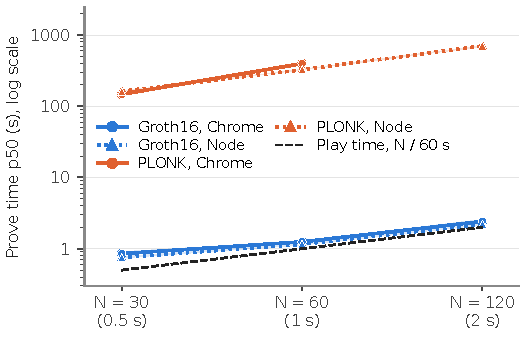
\includegraphics[width=\columnwidth]{figures/prove-time.pdf}
\caption{Prove time p50 against window size, with p5--p95 bands. Below the dashed line, proving keeps up with play. Sample counts are 1--20 per point. Chrome PLONK at $N=120$ has no point because its zkey failed to load.} % src: bench/RESULTS.md
\label{fig:prove}
\end{figure}

\begin{figure}[t]
\centering
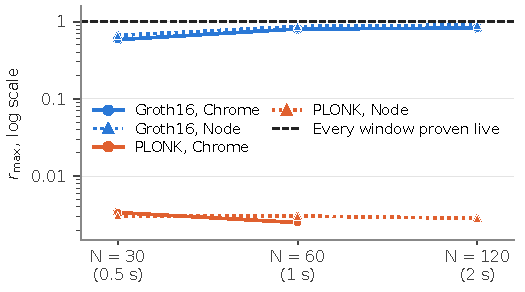
\includegraphics[width=\columnwidth]{figures/r-max.pdf}
\caption{Largest sustainable challenge rate $\rmax$ for one prover, computed as $(N/60\ \mathrm{s})$ divided by mean prove time.} % src: bench/RESULTS.md
\label{fig:rmax}
\end{figure}

Groth16 prove/play is above 1 for every variant (1.10--1.72), so one prover on this laptop cannot prove every window as fast as it is played. % src: docs/REPORT.md
This result is what motivates sampling plus a deferred audit.
Larger windows spread the fixed cost better (Node $\rmax$ 0.66, 0.86 and 0.91 for $N=30$, 60 and 120), but a challenged window takes longer to answer (2.2--2.4~s at $N=120$). % src: docs/REPORT.md
Verification takes 7--10~ms and proofs are about 723~B, whatever the value of $N$. % src: docs/REPORT.md
Chrome proves 9--13\% slower than Node, and witness generation is 5--8\% of proving time. % src: docs/REPORT.md

PLONK proves 170--320 times slower than Groth16 at the same $N$, with $\rmax$ near 0.003, so one second of play takes 5--7 minutes to prove. % src: docs/REPORT.md
That is too slow for spot-checks and for a post-match audit on this hardware.
Memory is also a hard limit: Chrome peaked at 15.1~GiB of the laptop's 16~GB at $N=60$, and the 3.96~GiB zkey at $N=120$ failed to load. % src: docs/REPORT.md
Its proofs are about 2.9 times larger, and verification time is similar. % src: docs/REPORT.md

\subsection{Detection Experiment}
We ran 135 matches with scripted cheats, using the real $N=60$ Groth16 circuit (\texttt{bench/out/detection.csv}, rows 1--135). % src: docs/REPORT.md
The Node matrix crossed speedhack, rapid-fire, infinite ammo and snap-aim with $m \in \{1, 5, 20\}$ cheated windows, with 10 runs each, and added 10 smooth-aim runs. % src: docs/REPORT.md
Two Node bots proved in worker threads on the same CPU. % src: docs/REPORT.md
A further five browser runs (one per cheat) used two Chrome windows. % src: docs/REPORT.md
Cheats were switched on from window 3. % src: docs/REPORT.md
Bots fire but always miss, to keep each match to one round. % src: docs/REPORT.md

All 124 rule-breaking runs (120 Node, 4 browser) ended \status{audited\_failed}. % src: docs/REPORT.md
In every run, every cheater window that broke a rule failed and every other window was valid, with the rule checker on the cheater's own tick log as ground truth. % src: docs/REPORT.md
We recomputed these counts and the latencies below from the CSV, and they match. % src: docs/REPORT.md

Table~\ref{tab:detection} compares live catches with two predictions. % src: n/a (structural count)
The naive estimate $1-(1-r)^m$ assumes that each window is checked independently with probability $r$. % src: docs/REPORT.md
At $m=1$ it predicts about 55\%, while 85\% were caught live. % src: docs/REPORT.md
The scheduler draws uniformly from all unproven windows of the round, so a window that ends early stays in the pool for many draws.
A Monte Carlo replay of each run's real challenge times predicts about 81\%, within the binomial margin of the observed rate. % src: docs/REPORT.md
The naive formula is therefore a lower bound and not a prediction.
The corollary is that windows near the end of a round are rarely checked live.
The six $m=1$ cheats missed live were all caught by the audit. % src: docs/REPORT.md

\begin{table}[t]
\centering
\caption{Live Catch Rate Against Predictions (Node Runs)}
\label{tab:detection}
\begin{tabular}{@{}rrrr@{}}
\toprule
$m$ & Caught live & Naive $1-(1-r)^m$ & Scheduler-aware \\ % src: docs/REPORT.md
\midrule
1 & 34/40 = 85\% & $\approx$ 55\% & $\approx$ 81\% \\ % src: docs/REPORT.md
5 & 40/40 = 100\% & 97--100\% & 100\% \\ % src: docs/REPORT.md
20 & 40/40 = 100\% & 100\% & 100\% \\ % src: docs/REPORT.md
\bottomrule
\end{tabular}
\end{table}

The 95\% confidence interval at $m=1$ is about 70--94\%. % src: docs/REPORT.md
Live detection latency, from switching the cheat on to the first failed spot-check, had a median of 4.5~s, p95 of 8.6~s and a maximum of 10.6~s over 114 Node catches. % src: docs/REPORT.md
Of these, 62 were caught in the activation window, and 113 within three windows. % src: docs/REPORT.md
The achieved challenge rate was $r \approx 0.49$ in honest play with Node provers and 0.34--0.65 with Chrome provers. % src: docs/REPORT.md
Per-configuration means rose to 0.53--0.85 while cheating, because a cheated window fails within milliseconds and the next challenge comes sooner. % src: docs/REPORT.md
Rapid-fire breaks a rule only when a shot falls inside the cooldown, so on average only 3.7 of 5 and 13 of 20 nominal windows actually broke a rule. % src: docs/REPORT.md

\subsection{Live Tests of 2026-10-23} % src: bench/out/screenshots/cheat-test-2026-10-23/README.md
We also ran browser bots through the full interface in private rooms, with cheats switched on through the development drawer. % src: bench/out/screenshots/cheat-test-2026-10-23/README.md
These demonstration runs are not part of the detection dataset (Table~\ref{tab:live}). % src: bench/out/screenshots/cheat-test-2026-10-23/README.md
A speedhack was first detected 3.38~s after activation and rapid-fire after 5.72~s. % src: bench/out/screenshots/cheat-test-2026-10-23/README.md
The honest player was \status{audited\_clean} in both runs, with 56/56 and 15/15 windows valid and no false positives. % src: bench/out/screenshots/cheat-test-2026-10-23/README.md
In run~A1 the cheater won through a forfeit that the test harness triggered, and the audit marked the result \status{overturned} (Fig.~\ref{fig:results}). % src: bench/out/screenshots/cheat-test-2026-10-23/README.md
A second test had both players cheat, with first detections at 9.43~s, 2.67~s and 3.91~s. % src: bench/out/screenshots/cheat-test-both-2026-10-23/README.md
No window failed while its player's cheat was off. % src: bench/out/screenshots/cheat-test-both-2026-10-23/README.md

\begin{table}[t]
\centering
\caption{Live Tests of 2026-10-23, $N=60$. A: Cheater vs Honest. B: Both Cheat. O: Observe, S: Strict. Lat.: Cheat On to First Detection.} % src: bench/out/screenshots/cheat-test-2026-10-23/README.md
\label{tab:live}
\setlength{\tabcolsep}{3pt}
\footnotesize
\begin{tabular}{@{}llrrrl@{}}
\toprule
Run & Player & Valid & Checks & Lat. & Own audit \\
\midrule
A1 O & speedhack & 50/56 & 24/29 & 3.38 s & failed \\ % src: bench/out/screenshots/cheat-test-2026-10-23/README.md
& honest & 56/56 & 25/25 & -- & clean \\ % src: bench/out/screenshots/cheat-test-2026-10-23/README.md
A2 S & rapid fire & 12/15 & 6/7 & 5.72 s & failed \\ % src: bench/out/screenshots/cheat-test-2026-10-23/README.md
& honest & 15/15 & 7/7 & -- & clean \\ % src: bench/out/screenshots/cheat-test-2026-10-23/README.md
B1 O & speedhack & 48/56 & 18/21 & 9.43 s & failed \\ % src: bench/out/screenshots/cheat-test-both-2026-10-23/README.md
& rapid fire & 50/56 & 18/21 & 2.67 s & failed \\ % src: bench/out/screenshots/cheat-test-both-2026-10-23/README.md
B2 S & speedhack & 5/8 & 3/4 & 3.91 s & failed \\ % src: bench/out/screenshots/cheat-test-both-2026-10-23/README.md
& rapid fire & 8/8 & 4/4 & -- & clean \\ % src: bench/out/screenshots/cheat-test-both-2026-10-23/README.md
\bottomrule
\end{tabular}
\end{table}

\begin{figure}[t]
\centering
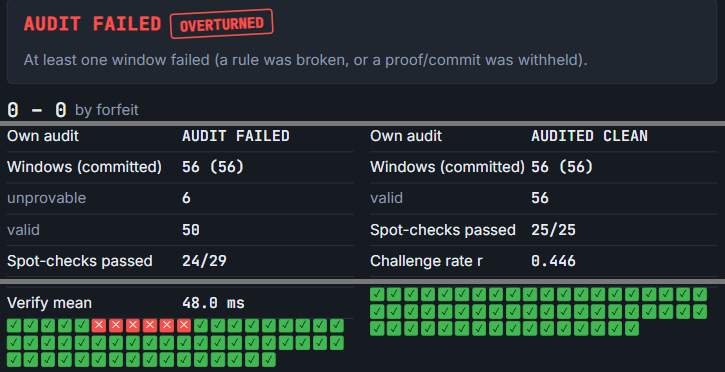
\includegraphics[width=\columnwidth]{figures/results-crop.png}
\caption{Results page of run A1, cropped to three bands: verdict, per-player audit rows and per-window proof strips. Cheater left, honest player right. The cheater's six failed windows are marked in red.} % src: bench/out/screenshots/cheat-test-2026-10-23/README.md
\label{fig:results}
\end{figure}

\subsection{Smooth-Aim Control}
Smooth-aim turns towards the target at or below the turn limit, so it breaks no proven rule.
It ended \status{audited\_clean} in 11/11 runs (10 Node, 1 browser). % src: docs/REPORT.md
This is the expected result: the control shows that the system does not flag rule-abiding automation, and also that it cannot detect such automation.

\subsection{Frame Time While Proving}
We measured the worst case: two Chrome windows on one laptop, each running a 12-thread prover, with the server on the same machine. % src: docs/REPORT.md
Frame interval p95 was 7.1~ms in Canvas 2D and 13.9~ms in the 3D renderer on a display of about 144~Hz, within our 20~ms requirement. % src: docs/REPORT.md
In a 3-minute honest match, 64/64 spot-checks passed ($r=0.36$), and the audit took 242~s with 180/180 windows valid per player. % src: docs/REPORT.md
With both provers sharing the CPU, a live spot-check proof took about 2.2~s on average (p95 2.8~s), against 1.25~s for one prover alone. % src: docs/REPORT.md
The audit is the visible cost: players wait about 2--4 minutes after a 3-minute match. % src: docs/REPORT.md

% ======================================================================
\section{Discussion and Limitations}
\label{sec:discussion}

\paragraph*{A false positive from outside the proof system}
Before release, honest matches failed with \status{mismatch\_digest}. % src: docs/CHANGELOG.md
The cause was a rate limiter counting snapshots in fixed intervals.
A brief browser stall produced a catch-up burst, the limiter dropped real snapshots, the server's digest then held stale values, and an honestly proven window failed. % src: docs/CHANGELOG.md
We replaced the limiter with token buckets and added a test that replays honest stall traces. % src: docs/CHANGELOG.md
Repeat matches then ended clean, and the detection dataset, which contains only \status{valid} and \status{unprovable} windows, was unaffected. % src: docs/CHANGELOG.md
The lesson is that a digest check turns any data loss on the server into an apparent proof failure.
Honest controls under realistic stalls are therefore as important as the cheat matrix.

\paragraph*{Smooth aim}
Proofs show compliance and not provenance, and this is the main limitation.
Any automation within the rules passes, and generated aimbots are designed to look human as well~\cite{kanervisto2023}.
We therefore argue for a hybrid: ZKPs for auditable rule claims, and server-side and behavioural detection for input provenance.
We have not built or evaluated such a hybrid.

\paragraph*{The final window}
A window cut off by the end of the match does not exist in the protocol, so nothing in it is proven.
In run B2, the rapid-fire player fired illegally in window 8, but the match ended in that window when the opponent forfeited on a failed spot-check. % src: bench/out/screenshots/cheat-test-both-2026-10-23/README.md
That player committed only honest windows, was \status{audited\_clean} and was recorded as a \status{verified} winner, although the cheat flag was logged. % src: bench/out/screenshots/cheat-test-both-2026-10-23/README.md
Run B1 shows a related rule: when both players fail, the verdict considers only the recorded winner, and no new winner is picked. % src: bench/out/screenshots/cheat-test-both-2026-10-23/README.md

\paragraph*{Single-party setup}
Phase 2 of the Groth16 setup is one local contribution, so whoever ran it could in principle forge proofs. % src: docs/REPORT.md
A deployment would need a multi-party ceremony or a transparent or universal scheme, and PLONK is impractical here.

\paragraph*{One machine}
All numbers come from one mid-range laptop, and the planned run on a stronger machine was not done. % src: docs/REPORT.md
Every two-player measurement shared one CPU, which is pessimistic for proving. % src: docs/REPORT.md
Node provers are about 1.2 times faster than Chrome, so $r$ in the Node matrix is somewhat higher than two browsers would reach. % src: docs/REPORT.md

\paragraph*{Small PLONK samples}
PLONK has 1--5 samples per variant, and Chrome at $N=60$ is a single proof, so its numbers are less precise than those for Groth16. % src: docs/REPORT.md
The conclusion rests on a gap of two orders of magnitude. % src: docs/REPORT.md

\paragraph*{Scope of the evidence}
Our cheats are scripted and our bots always miss, with a fixed activation window, and browser detection runs are single runs per cheat. % src: docs/REPORT.md
We make no claim about human cheaters or commercial titles.
A disconnect makes the rest of a round \status{chain\_broken}, which limits the audit to \status{audit\_incomplete}: visible, but not proof of cheating.

% ======================================================================
\section{Conclusion and Future Work}

We presented a commit--challenge--audit protocol and a working browser implementation that proves per-tick movement, aim and weapon rules over committed hidden state.
On a mid-range laptop, Groth16 cannot prove every window in real time, but it is usable with sampling and a deferred audit, while PLONK is impractical.
In our experiment, every rule-breaking cheat ended \status{audited\_failed} and most were caught live within seconds; in the live tests, every window of the honest player verified.
A rule-abiding aimbot passed, which marks the boundary of what such proofs can claim.

Future work includes closing the final-window gap, a multi-party setup, measurements on stronger hardware and across a real network, other proof systems, interior walls in the circuit and an evaluation of the proposed hybrid with behavioural detection.

\balance
\bibliographystyle{IEEEtran}
\bibliography{refs}

\end{document}
